% IEEE BigData 2026 -- Special Session on Machine Learning on Big Data
% Compile with pdflatex + bibtex (IEEEtran.cls V1.8b, IEEEtran.bst V1.14).
\documentclass[conference]{IEEEtran}
\IEEEoverridecommandlockouts
\usepackage{cite}
\usepackage{amsmath,amssymb}
\usepackage{graphicx}
\usepackage{booktabs}
\usepackage{array}
\usepackage{url}
\usepackage[hidelinks]{hyperref}

\newcommand{\Yold}{Y^{\mathrm{old}}}
\newcommand{\Ycur}{Y^{\mathrm{cur}}}

\begin{document}

\title{Relevance-Label Revisions in PinPoint:\\
A Fixed-Output Audit of Two Public Releases}

\author{\IEEEauthorblockN{Ziang Tan}
\IEEEauthorblockA{\textit{Department of Electrical and Computer Engineering} \\
\textit{University of Washington}\\
Seattle, WA, USA \\
ziangt2@uw.edu}}

\maketitle

\begin{abstract}
When a benchmark's relevance labels are revised, a common check is whether system order survives. We ask what that check misses. Using PinPoint, a composed image retrieval benchmark, we rescore the same cached outputs of seven released runs under the labels of its first public data commit and of its current release, holding requests, candidate domain and metric code fixed. Two findings stand out. First, the point order of all seven runs is unchanged, but the S1 reranking advantage falls from 0.043 to 0.023 (paired change $-0.020$, 95\% interval $[-0.031,-0.010]$), and the absolute advantage also roughly halves across all 4,225 queries whose instructions and reference-image IDs are unchanged. Second, the public evaluator's paraphrase-sensitivity metric, which we reproduce exactly, reorders the runs although no output changes (Kendall $\tau=0.33$), and a run that ignores the wording acquires a nonzero value. The revision is traceable to a label replacement after which 121 of 344 matched groups that we construct no longer share one positive set. These results concern evaluation values under two public label versions; they do not establish which labels are correct, why they changed, or whether conclusions of the original benchmark paper hold.
\end{abstract}

\begin{IEEEkeywords}
benchmark versioning, relevance judgments, data provenance, evaluation reliability, composed image retrieval
\end{IEEEkeywords}

%======================================================================
\section{Introduction}
%======================================================================
Machine learning progress is increasingly reported against public benchmarks distributed through code repositories and data hubs. These benchmarks change after release: maintainers fix annotations, relicense content, and replace candidate pools, and each revision can change the labels against which later models are scored. This raises a provenance question for large-scale evaluation: \emph{when a benchmark's labels change but its requests do not, which conclusions drawn from earlier scores still hold?}

Information retrieval (IR) research has long studied how alternative relevance judgments affect evaluation. Substituting assessors changes absolute scores while largely preserving system rankings~\cite{voorhees2000,sanderson2005}, incomplete judgments and pooling bias affect comparisons~\cite{zobel1998,buckley2004}, recent reannotations revisit these questions for neural rankers~\cite{parry2025,arabzadeh2022}, and corrected test sets can reorder models~\cite{northcutt2021,beyer2020}. A common way to use this knowledge is to check whether system order survives a change in judgments. That check cannot tell whether the \emph{size} of a reported improvement, or a robustness score computed from variation \emph{within} groups of queries, keeps its meaning. Answering these questions requires holding model outputs fixed while labels change along an actual release history. This is the setting we study.

We audit one such history in PinPoint~\cite{pinpoint}, a composed image retrieval (CIR) benchmark with multiple positives, explicit negatives, multi-image queries and paraphrase testing. The PinPoint paper states that each paraphrase shares the same positive and negative annotations, so that quality variation across paraphrases measures sensitivity to wording. Three objects must be kept apart (Table~\ref{tab:objects}): this protocol, the public evaluator code, which groups rows by reference-image signatures, and the matched groups we construct for the audit. We rescore the \emph{same} cached rankings of seven released runs under old and current labels with requests, candidate domain and metric code fixed, so every score difference is attributable to the label version.

Our central observation is that \textbf{system order stays the same while two quantities that researchers interpret change}. The first is the \emph{size of an improvement}: the S1 reranking stage still helps under both label versions, but its estimated benefit roughly halves, in the matched groups and among all queries whose requests are unchanged (Fig.~\ref{fig:main}a). The second is the \emph{sensitivity ordering} reported by the benchmark's own evaluator: with outputs fixed, the runs are ordered differently by paraphrase sensitivity, and a run that cannot respond to wording acquires a nonzero value (Fig.~\ref{fig:main}b). Fig.~\ref{fig:design}b shows the underlying mechanism in one real group: replacing a positive list changes scores and creates within-group variation without any change in outputs.

\textbf{Main findings.}
\begin{itemize}
\item \emph{Improvement sizes differ across label versions.} The S1 reranking advantage falls from 0.043 to 0.023 while the point order of all seven runs is preserved; the absolute halving extends beyond our matched groups to all 4,225 unchanged queries (Secs.~\ref{sec:res-quality}--\ref{sec:res-scaling}).
\item \emph{The benchmark's sensitivity ordering changes with fixed outputs.} Using a re-implementation that reproduces the published evaluator values exactly, the ordering of runs by within-group P@10 range changes (Kendall $\tau=0.33$), and a wording-blind run moves from zero to a nonzero value (Secs.~\ref{sec:res-range}--\ref{sec:res-evaluator}).
\end{itemize}
The release-chain tracing (Sec.~\ref{sec:res-split}) provides the context for these findings. A proportional-scaling test, leave-one-component-out analysis and domain and normalization checks qualify them, and a released package regenerates every table, figure and quoted number from pinned public inputs (Data and Code Availability section). The four-cell report and missing-rank bounds are analysis tools, not proposed evaluation methods.

\begin{table}[!t]
\centering
\caption{Protocol, public implementation and the matched groups of this audit.}
\label{tab:objects}
\footnotesize
\setlength{\tabcolsep}{3pt}
\begin{tabular}{@{}>{\raggedright\arraybackslash}p{0.2\columnwidth}>{\raggedright\arraybackslash}p{0.47\columnwidth}>{\raggedright\arraybackslash}p{0.27\columnwidth}@{}}
\toprule
Object & Grouping and scoring & Role here\\
\midrule
PinPoint paper~\cite{pinpoint} (Secs.~3.1.2, 4.1.2) & Paraphrases share positive and negative annotations; sensitivity is the range of mAP@10 across a query's paraphrases, averaged over queries & Stated evaluation condition\\
Public evaluator code & Rows grouped by reference-image signature pair; range of P@10 within a group & Observed implementation\\
Matched groups (this paper) & Old rows sharing a normalized reference pair \emph{and} an identical old positive set; complete, with unchanged references & Controlled population for the audit\\
\bottomrule
\end{tabular}
\end{table}

%======================================================================
\section{Related Work}
%======================================================================
\textbf{Relevance-judgment variation.} Voorhees~\cite{voorhees2000} showed that substituting one assessor's judgments for another's changes absolute scores while leaving TREC system rankings largely stable. Zobel~\cite{zobel1998} and Buckley and Voorhees~\cite{buckley2004} studied pooling bias and incomplete judgments, Sanderson and Zobel~\cite{sanderson2005} related judgment effort to the reliability of significance conclusions, and Smucker et al.~\cite{smucker2007} compared significance tests for IR. For neural rankers, Arabzadeh et al.~\cite{arabzadeh2022} found that sparse MS MARCO labels can rate a strong system below its preferred quality, and Parry et al.~\cite{parry2025} reannotated TREC DL topics~\cite{trecdl2019} to measure the shelf life of test collections. These studies mostly vary who judges and report score levels, rank correlations or significance conclusions. Our evidence adds a specific combination: an actual release history of one benchmark, outputs held fixed, and the effect of the revision on a paired improvement and on within-group score variation.

\textbf{Label errors and benchmark reliability.} Northcutt et al.~\cite{northcutt2021} estimated label errors in popular test sets and showed that corrections can reorder models; Beyer et al.~\cite{beyer2020} reassessed ImageNet labels, and Recht et al.~\cite{recht2019} measured accuracy drops on a reconstructed test set. Here the revision is made by the maintainers and affects a structural property, label sharing within groups, on which a robustness metric depends.

\textbf{Dataset documentation and versioning.} Datasheets~\cite{gebru2021} and data cards~\cite{pushkarna2022} call for documenting dataset collection and maintenance, Koch et al.~\cite{koch2021} documented how research concentrates on a few reused datasets, and Longjohn et al.~\cite{longjohn2024} recommended version identifiers and revision records in benchmark repositories. Our audit shows what such identifiers would reveal in practice.

\textbf{CIR and paraphrase robustness.} CIR benchmarks such as Fashion-IQ~\cite{fashioniq}, CIRR~\cite{cirr} and CIRCO~\cite{circo} score rankings for a reference image plus modifying text~\cite{tirg}. Query-variation robustness is typically measured through score or rank consistency across variants~\cite{penha2022,prsm}; such measures assume the relevance target is shared across variants, which is the premise our audit examines.

%======================================================================
\section{Audit Design}\label{sec:method}
%======================================================================
\subsection{Notation and analysis tool}
Let $R_q$ be a system's ordered output for query $q$, $Y_q$ a label version and $C$ a candidate domain. The label-version effect on metric $f$ is $\Delta_q=f(R_q,\Ycur_q,C)-f(R_q,\Yold_q,C)$ with $R_q$ and $C$ fixed. It is neither a label-error rate nor model deterioration.

When outputs and labels both differ, the four cells $f_{ij}=f(R_i,Y_j,C)$ satisfy the accounting identity
\begin{equation}\label{eq:four}
f_{11}-f_{00} = O_0 + L_0 + I,
\end{equation}
with output change $O_0=f_{10}-f_{00}$, label change $L_0=f_{01}-f_{00}$ and interaction $I=f_{11}-f_{10}-f_{01}+f_{00}$. We use it only for bookkeeping: when $I\neq0$, the order of substitution changes the components, so it is not a causal attribution. The released report prints all four cells, both substitution orders and label-free output diagnostics, and rejects rankings shorter than the metric depth or containing duplicate IDs.

\subsection{Releases and matched groups}\label{sec:frame}
The \emph{old} labels are those of the first public data commit of the PinPoint repository (\texttt{1dd9d69}, November 2025), which remained unchanged until commit \texttt{5fc977b} (February 2026, message ``updates signatures and metrics''). The \emph{current} labels are those of revision \texttt{059d6e4}, whose label file was last modified in March 2026. Old rows sharing a normalized reference-image pair and an identical positive set form a group; we keep groups with at least two queries. Of 1,298 such groups (from 7,846 old rows), 134 lose one or more rows in the current release, and 820 of the remaining 1,164 change a reference signature. The audit frame contains \textbf{344 groups and 2,091 queries}, each query keeping its instruction and reference-image IDs in both releases. Selection never uses model scores.

These groups are a matched population defined by artifact consistency. They are neither a random sample of PinPoint nor verified sets of equivalent intents, and they need not coincide with the paraphrase sets of the original protocol or with the public evaluator's groups.

\begin{figure*}[!t]
\centering
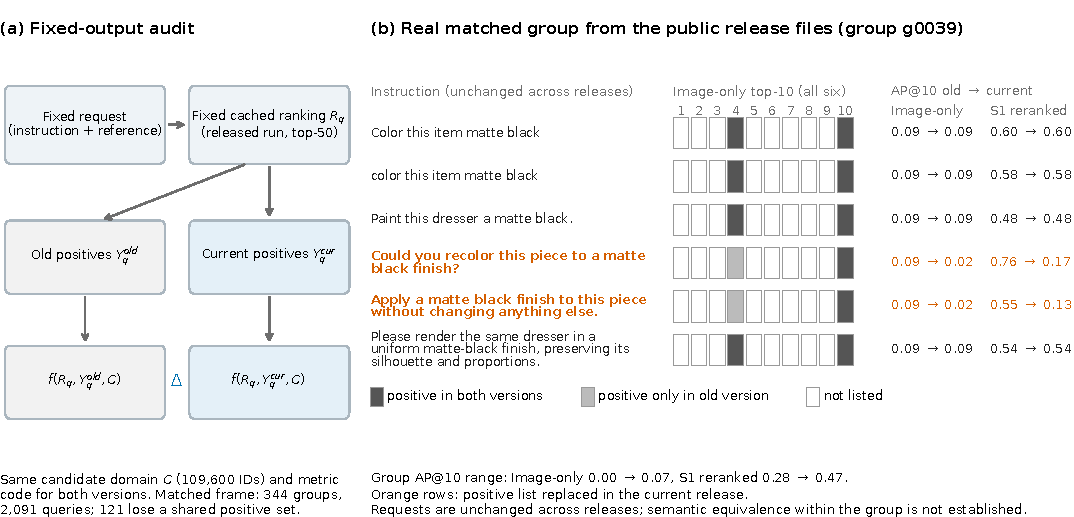
\includegraphics[width=\textwidth]{figures/fig1_design_case.pdf}
\caption{(a) Audit design: one cached ranking is scored under two label versions with request, candidate domain and metric fixed, so any score difference is a label-version effect. (b) Matched group \texttt{g0039} from the public release files, chosen by a fixed rule (Sec.~\ref{sec:res-split}). All six requests share one reference image and, for MetaCLIP2 Image-only, one top-10 ranking. Requests are unchanged across releases; semantic equivalence within the group is not established. Two requests (orange) had their positive list replaced; the item at rank 4 is no longer a positive for them, so their scores drop and a within-group range appears although no output changed. The figure reports file contents; it does not judge which list is correct. The overall findings are shown in Fig.~\ref{fig:main}.}
\label{fig:design}
\end{figure*}

\subsection{Fixed outputs and replaced labels}
We use all seven released cached runs compatible with the current index: two BGE-VL MLLM checkpoints~\cite{megapairs} (S1 and S2), S1 followed by the released reranking stage (S1 reranked), and four MetaCLIP2~\cite{metaclip2} variants (Combined, Image-only, Text-only and SLERP interpolation). Names follow the release files; the caches do not certify historical checkpoints or configurations. Each run supplies an ordered top-50 list per query. In the primary analysis the candidate domain $C$ is the set of 109,600 current index IDs for both label versions; we project each version's positive list onto $C$, retaining duplicates, and rescore the unchanged ranking. Scoring old labels on current caches answers a controlled substitution question; it does not reproduce historical native inference.

\subsection{Metrics and statistical units}
We follow the public evaluator: AP@10 counts a hit by set membership and divides by the raw positive-list length,
\begin{equation}\label{eq:ap}
\mathrm{AP@10}(R_q,Y_q)=\frac{\sum_{i=1}^{10} h_{qi}\,\frac{1}{i}\sum_{j=1}^{i}h_{qj}}{\min(10,|Y_q|)},
\end{equation}
where $h_{qi}=\mathbf 1\{R_q(i)\in\mathrm{set}(Y_q)\}$, and P@10 is the top-10 hit count divided by 10. Unlisted candidates score zero without being treated as judged negatives, and queries without projected positives score zero and stay in the population (none occur in the primary frame). Quality is averaged over queries. Group fluctuation is the within-group range averaged equally over groups:
\begin{equation}\label{eq:range}
\overline G(Y)=\frac{1}{|\mathcal G|}\sum_{g\in\mathcal G}\Big[\max_{q\in g}f(R_q,Y_q)-\min_{q\in g}f(R_q,Y_q)\Big].
\end{equation}

Paired intervals use 5,000 percentile-bootstrap draws~\cite{efron1993} over the 312 connected components of queries that share reference images (largest component: 30 queries; seed 20260920); strata keep the components of the full frame that they intersect. This respects the modeled reference dependence but not every shared-candidate relation. Because earlier release observations informed the design, all analyses are exploratory, and intervals are unadjusted for multiplicity.

\subsection{Common-candidate diagnostic}
To check that results do not depend on the candidate domain, we also score on the 30,535 IDs present in both releases. Filtering a cached top-50 list yields an exact top-10 only when at least ten entries survive; this holds for all seven runs in 271 groups (1,636 queries). For all 344 groups we also report missing-tail bounds, obtained by assuming that unknown ranks contain no positives (lower) or the remaining projected positives first (upper). They are identification bounds, not confidence intervals.

%======================================================================
\section{Results}\label{sec:results}
%======================================================================
\subsection{A shared positive set splits within unchanged requests}\label{sec:res-split}
At the first positive-list replacement (\texttt{5fc977b}), \textbf{121 of the 344 matched groups} no longer share one positive set; the count is the same in the current release. In 119 of them some rows keep their old positives, and in two all rows change. Every split group now carries exactly two distinct positive sets. Negative lists change less: projected onto the current domain, all 344 groups share one negative set in the old release and 292 in the current one. All 121 remain split after projection onto the common candidate domain, so candidate-pool changes alone do not explain the divergence. The other 223 groups contain 323 rows whose positive lists also changed without breaking set equality within the group; they are a complementary stratum, not an unchanged-label control.

\textbf{A real case.} Fig.~\ref{fig:design}b shows group \texttt{g0039}, selected by a rule fixed before drawing the figure: among the 44 split groups in which the Image-only top-10 contains an item whose positive status differs between versions, sort by current Image-only range (ties broken by group identifier) and take the lower median, i.e.\ the 22nd group; there is no tie at this position. The group has six requests about a matte-black finish with one reference image; each request's instruction and reference-image ID are identical in both releases. The requests differ in wording and, in two cases, in added constraints, and we do not establish that they are semantically equivalent. In the first public data commit all six requests share five positives. In the current release, two requests (``Could you recolor this piece to a matte black finish?'' and ``Apply a matte black finish to this piece without changing anything else.'') keep one of the five and gain two new IDs, one of which is listed three times; the other four requests are unchanged. The Image-only ranking, identical for all six requests, has an old positive at rank 4 that is no longer a positive for those two requests, so their AP@10 falls from 0.09 to 0.02 and the group range rises from 0 to 0.07. For S1 reranked, whose rankings differ across requests, the two affected requests fall from 0.76 to 0.17 and from 0.55 to 0.13.

The case is typical in structure but not in every detail. Of the 121 split groups, 116 contain six queries, the number of paraphrases per request in PinPoint's protocol, although we do not verify that they are the protocol's paraphrase sets; between one and six rows change per group (median Jaccard overlap of changed lists 0.21, 68 of 349 with no overlap). Duplicated positive IDs appear only after the revision: 1,114 of the 7,635 current rows contain them, against none of the 7,846 old rows. The commit history records that data files changed, but the commit messages do not describe label replacements. We document what the public files contain; we do not judge which list is correct, why it changed, or how many paraphrase sets of the original protocol are affected.

\subsection{Order is preserved, but the reranking benefit halves}\label{sec:res-quality}
Under current labels, query-mean AP@10 decreases for every run by 0.016--0.084, or 24--32\% (Table~\ref{tab:quality}, Fig.~\ref{fig:quality}); P@10 decreases by 19--20\%. The point order of the seven runs is identical under both versions for both metrics, although MetaCLIP2 Combined and SLERP are effectively tied (AP@10 margin 0.0009 old, 0.0004 current). A ranking check would therefore report no change.

\begin{table}[!t]
\centering
\caption{Query-mean quality under old and current labels (current candidate domain, 344 groups, 2,091 queries). $\Delta$ = current $-$ old with paired 95\% component-bootstrap interval.}
\label{tab:quality}
\setlength{\tabcolsep}{3.2pt}
\footnotesize
\begin{tabular}{@{}lccccc@{}}
\toprule
 & \multicolumn{3}{c}{AP@10} & \multicolumn{2}{c}{P@10}\\
\cmidrule(lr){2-4}\cmidrule(l){5-6}
Run & Old & Cur. & $\Delta$ [95\% CI] & Old & Cur.\\
\midrule
S1 reranked & .3069 & .2226 & $-.0843$ [$-.105$, $-.066$] & .2834 & .2272\\
S1 & .2641 & .1999 & $-.0641$ [$-.082$, $-.048$] & .2448 & .1986\\
S2 & .2420 & .1785 & $-.0635$ [$-.081$, $-.048$] & .2411 & .1946\\
MC2 Combined & .1465 & .1041 & $-.0424$ [$-.055$, $-.031$] & .1771 & .1416\\
MC2 SLERP & .1456 & .1038 & $-.0419$ [$-.055$, $-.030$] & .1844 & .1473\\
MC2 Text-only & .1035 & .0706 & $-.0329$ [$-.045$, $-.022$] & .1112 & .0887\\
MC2 Image-only & .0664 & .0505 & $-.0158$ [$-.022$, $-.011$] & .1009 & .0807\\
\bottomrule
\end{tabular}
\\[2pt]\raggedright\scriptsize MC2 = MetaCLIP2. Rows sorted by old AP@10; the order is identical under current labels.
\end{table}

\begin{figure}[!t]
\centering
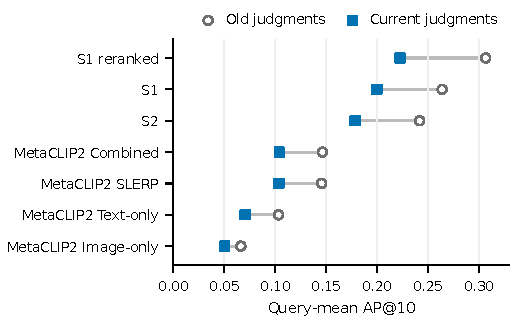
\includegraphics[width=\columnwidth]{figures/fig2_quality.pdf}
\caption{Query-mean AP@10 of seven cached runs under old and current labels. Rankings are identical across conditions; every shift is a label-version effect.}
\label{fig:quality}
\end{figure}

The size of an improvement is a different matter. The advantage of S1 reranked over S1 falls from 0.0428 (95\% interval $[0.024, 0.061]$) under old labels to 0.0226 ($[0.007, 0.038]$) under current labels. The paired change is $-0.0201$ ($[-0.0312, -0.0100]$), a 47\% relative reduction and a ratio of 0.53 (Fig.~\ref{fig:main}a). Reranking still helps under both versions, but a benefit estimated under one label version does not transfer to the other. In the four-cell bookkeeping of Eq.~\eqref{eq:four}, with $f_{00}=0.2641$, $f_{10}=0.3069$, $f_{01}=0.1999$ and $f_{11}=0.2226$, the interaction $I=-0.0201$ equals this change in advantage, while the two pipelines differ in all 2,091 ordered top-10 lists (mean top-10 non-overlap 0.608).

\begin{figure*}[!t]
\centering
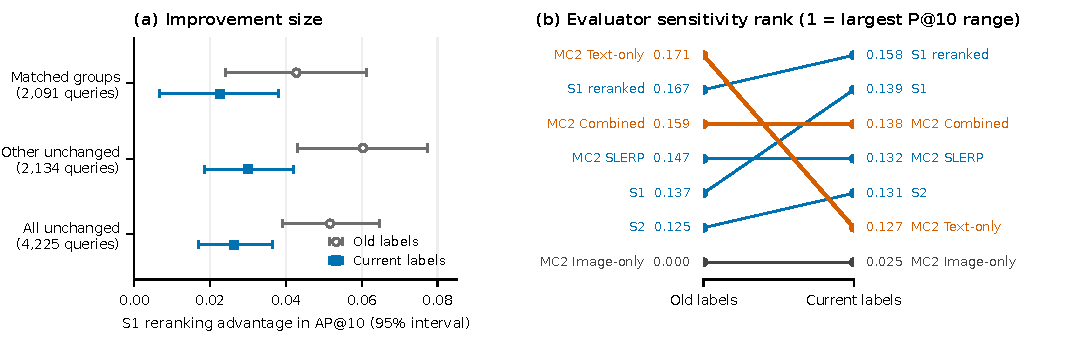
\includegraphics[width=\textwidth]{figures/fig3_main_findings.pdf}
\caption{The two main findings, both with model outputs held fixed. (a) S1 reranking advantage in AP@10 under old and current labels with paired 95\% component-bootstrap intervals, for the matched groups, the other unchanged queries and all 4,225 queries whose instructions and reference-image IDs are unchanged (Table~\ref{tab:scaling}). (b) Ranks of the seven runs under the public evaluator's sensitivity metric (mean within-group P@10 range over rows grouped by reference-image signature; values next to names; a lower value means a smaller metric value), on the same 4,225 unchanged rows (Table~\ref{tab:evaluator}). Rank changes are point estimates; orange marks the only pair whose difference changes sign with 95\% intervals excluding zero under both label versions.}
\label{fig:main}
\end{figure*}

\textbf{Supporting evidence: margins compress.} The reranking change is part of a broader pattern. All 21 pairwise AP@10 margins keep their sign and shrink in magnitude, to a median of 0.75 of their old size; for 19 of them the paired interval of the change excludes zero (unadjusted), the exceptions being S1 vs.\ S2 and the tied Combined vs.\ SLERP pair. P@10 shows the same pattern (20 of 21 margins shrink; 19 intervals exclude zero). Because the 21 pairs are built from the same seven runs and queries, they describe one pattern rather than 21 independent confirmations. A median ratio close to the per-run score ratios (0.68--0.76) indicates that most of the compression is consistent with an approximately proportional rescaling; the reranking advantage (ratio 0.53) shrinks more, while the advantage of S1 over MetaCLIP2 Combined shrinks roughly proportionally, from 0.118 to 0.096.

\subsection{Is the smaller benefit more than a rescaling, and does it extend beyond the matched groups?}\label{sec:res-scaling}
Because S1 itself loses about a quarter of its score, a smaller absolute advantage could simply reflect a smaller scale. We added three analyses to test this (Table~\ref{tab:scaling}). They were specified after the main analysis, use the same component bootstrap, and are reported with unadjusted intervals.

\textbf{Proportional scaling.} In the matched frame the relative gain of reranking, $(\mathrm{AP}_{\text{S1 reranked}}-\mathrm{AP}_{\text{S1}})/\mathrm{AP}_{\text{S1}}$, falls from 16.2\% to 11.3\% (paired change $-4.9$ points, $[-9.7, -0.2]$). If the advantage had fallen in proportion to the S1 score, the current advantage would be 0.032; the observed 0.023 lies below it by $-0.0097$ ($[-0.0193, -0.0005]$). Both intervals exclude zero, but only narrowly, and the two statistics are closely related rather than independent confirmations. Within the matched frame, the evidence therefore favors a reduction beyond proportional rescaling, with modest precision.

\textbf{Beyond the matched groups.} A wider sample contains every query present in both releases whose instruction and reference-image IDs are unchanged, with complete caches for all seven runs, without any grouping or shared-positive requirement: 4,225 queries, the 2,091 frame queries plus 2,134 others (1,801 of the 4,225 have a changed positive set). In this sample the point order of all seven runs is again unchanged, every run loses 35--40\% of its AP@10, and the absolute reranking advantage roughly halves both overall (0.052 to 0.026) and outside the frame (0.060 to 0.030). Outside the frame, however, the relative gain barely moves (27.2\% to 26.0\%, change $-1.2$ points, $[-8.3, 6.3]$) and the deviation from proportional scaling is $-0.0014$ ($[-0.0099, 0.0070]$). The halving of the absolute benefit thus extends to all unchanged queries, whereas a reduction beyond rescaling is observed in the matched groups but not established among the other unchanged queries. This comparison cannot isolate the cause, so we do not attribute the difference to the splitting of shared positive sets.

\textbf{Concentration.} The change in reranking advantage in the frame is not driven by a few reference-image components. Of 312 components, 180 contribute nothing, and the five with the largest absolute contribution account for 19\% of the total absolute contribution. Leaving out any single component keeps the change between $-0.022$ and $-0.018$ and the deviation from proportional scaling between $-0.0115$ and $-0.0082$; leaving out the top five together gives $-0.016$.

\begin{table*}[!t]
\centering
\caption{S1 reranking advantage in AP@10: absolute change, relative gain and deviation from proportional scaling (current $-$ expected if the advantage fell in proportion to S1). Paired 95\% component-bootstrap intervals, unadjusted; analyses added after the main analysis.}
\label{tab:scaling}
\footnotesize
\setlength{\tabcolsep}{2.6pt}
\begin{tabular}{@{}lrrcccccc@{}}
\toprule
 & & & \multicolumn{3}{c}{Advantage} & \multicolumn{2}{c}{Relative gain (\%)} & Deviation from\\
\cmidrule(lr){4-6}\cmidrule(lr){7-8}
Population & Queries & Comp. & Old & Cur. & $\Delta$ [95\% CI] & Old $\rightarrow$ cur. & $\Delta$ (points) [95\% CI] & proportional [95\% CI]\\
\midrule
Matched frame (344 groups) & 2,091 & 312 & 0.043 & 0.023 & $-$0.020 [$-$0.031, $-$0.010] & 16.2 $\rightarrow$ 11.3 & $-$4.9 [$-$9.7, $-$0.2] & $-$0.0097 [$-$0.0193, $-$0.0005]\\
Other unchanged queries & 2,134 & 448 & 0.060 & 0.030 & $-$0.030 [$-$0.042, $-$0.019] & 27.2 $\rightarrow$ 26.0 & $-$1.2 [$-$8.3, 6.3] & $-$0.0014 [$-$0.0099, 0.0070]\\
All unchanged queries & 4,225 & 690 & 0.052 & 0.026 & $-$0.025 [$-$0.033, $-$0.018] & 21.3 $\rightarrow$ 16.8 & $-$4.5 [$-$8.7, $-$0.4] & $-$0.0071 [$-$0.0140, $-$0.0006]\\
\bottomrule
\end{tabular}
\end{table*}

\subsection{Sensitivity appears without any change in outputs}\label{sec:res-range}
Within-group score ranges are the quantity behind paraphrase sensitivity. Their mean changes in opposite directions across strata (Fig.~\ref{fig:ranges}). For S1, the range decreases from 0.231 to 0.213 over all 344 groups ($\Delta=-0.018$, $[-0.035,-0.002]$), but increases from 0.201 to 0.234 in the 121 split groups ($+0.032$, $[0.005, 0.061]$) and decreases from 0.247 to 0.202 in the other 223 groups ($-0.046$, $[-0.065,-0.027]$). An aggregate sensitivity number therefore averages over opposing label-driven movements.

MetaCLIP2 Image-only makes the interpretation problem explicit. It scores candidates from the reference images alone, so all queries in a matched group receive the same ranking. Under old labels its range is exactly zero, because group members share both the positive set and the AP denominator. Under current labels its range becomes 0.014 overall ($[0.009, 0.019]$) and 0.039 in split groups ($[0.026, 0.053]$), and remains zero elsewhere. A run that cannot respond to wording thus acquires a nonzero wording ``sensitivity'' (Fig.~\ref{fig:design}b). Conversely, a split does not force unequal scores: replaced items may not be retrieved, or different hit patterns may tie. Across label versions, ranking change is exactly zero for every run, so none of these range changes reflects a change in model behavior.

\begin{figure*}[!t]
\centering
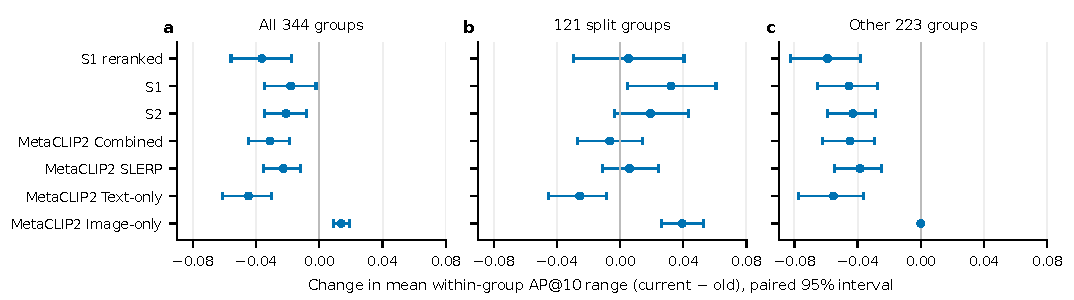
\includegraphics[width=\textwidth]{figures/fig4_ranges.pdf}
\caption{Change in mean within-group AP@10 range (current $-$ old) with paired 95\% component-bootstrap intervals, for (a) all matched groups, (b) the 121 groups whose positive set split, and (c) the remaining 223 groups. Rankings and candidate domain are fixed. The Image-only old range is zero by construction; stratum (c) is not an unchanged-label control.}
\label{fig:ranges}
\end{figure*}

\subsection{Consequences for the benchmark's reported sensitivity metric}\label{sec:res-evaluator}
The analyses above use our matched groups and the paper's AP-based range. The public evaluator reports a different quantity, the mean within-group P@10 range over rows grouped by reference-image signatures (Table~\ref{tab:objects}). We re-implemented it and first checked that it reproduces the repository's published \texttt{metrics.csv} exactly: all 21 values (mAP@10, P@10 and \texttt{ling\_sens\_range} for the seven runs) agree to the four published decimals. We then applied it, with outputs and grouping fixed, to all 4,225 rows whose instruction and reference-image IDs are unchanged (848 evaluator groups, 671 bootstrap components), switching only the positive lists. This analysis does not depend on our matched groups.

Table~\ref{tab:evaluator} and Fig.~\ref{fig:main}b show the result. The Image-only run, which cannot respond to wording, has a sensitivity of 0 under old labels and 0.0255 ($[0.0198, 0.0314]$) under current labels. The ordering of runs by sensitivity changes substantially (Kendall $\tau=0.33$ between the two orderings; $\tau=0.62$ for the AP-based range). MetaCLIP2 Text-only moves from the most sensitive run (0.171) to the second least sensitive (0.127; change $-0.043$, $[-0.052, -0.035]$). Of the 7 run pairs whose sensitivity difference changes sign, one has intervals excluding zero under both label versions (MetaCLIP2 Combined vs.\ Text-only); the others involve at least one difference that is not distinguishable from zero. A conclusion such as ``model A is more robust to paraphrasing than model B'' can therefore depend on the label version even when no output changes.

\begin{table}[!t]
\centering
\caption{The public evaluator's sensitivity metric (mean within-group P@10 range, groups by reference-image signature) with fixed outputs and grouping, 4,225 unchanged rows. Change: current $-$ old, paired 95\% interval. Rank: 1 = most sensitive.}
\label{tab:evaluator}
\footnotesize
\setlength{\tabcolsep}{3.5pt}
\begin{tabular}{@{}lcccc@{}}
\toprule
Run & Old & Cur. & Change [95\% CI] & Rank\\
\midrule
S1 reranked & .1671 & .1584 & $-$.0087 [$-$.0166, $-$.0005] & 2 $\rightarrow$ 1\\
S1 & .1367 & .1390 & +.0024 [$-$.0056, +.0104] & 5 $\rightarrow$ 2\\
S2 & .1245 & .1314 & +.0068 [$-$.0011, +.0147] & 6 $\rightarrow$ 5\\
MC2 Combined & .1594 & .1384 & $-$.0210 [$-$.0289, $-$.0131] & 3 $\rightarrow$ 3\\
MC2 SLERP & .1472 & .1324 & $-$.0147 [$-$.0223, $-$.0068] & 4 $\rightarrow$ 4\\
MC2 Text-only & .1708 & .1275 & $-$.0433 [$-$.0516, $-$.0352] & 1 $\rightarrow$ 6\\
MC2 Image-only & .0000 & .0255 & +.0255 [+.0198, +.0314] & 7 $\rightarrow$ 7\\
\bottomrule
\end{tabular}
\end{table}

\subsection{Robustness checks}\label{sec:res-checks}
\textbf{Candidate domain.} On the common candidate domain (Table~\ref{tab:common}), the exact 271-group subset shows the same direction of change and the same point order, and for all 344 groups every run's upper bound on the AP@10 change is negative.

\textbf{Normalization.} Using the number of \emph{unique} positives as the AP denominator, which removes the effect of duplicated IDs, raises current AP by only 0.0005--0.0018, so the evaluator's normalization does not explain the label effect.

\begin{table}[!t]
\centering
\caption{AP@10 change on the common candidate domain (30,535 IDs). Exact subset: 271 groups, 1,636 queries, paired 95\% interval. Bounds: all 344 groups, missing-tail identification bounds (not confidence intervals).}
\label{tab:common}
\setlength{\tabcolsep}{4pt}
\footnotesize
\begin{tabular}{@{}lccc@{}}
\toprule
Run & Exact $\Delta$ & 95\% CI & Full-frame bounds\\
\midrule
S1 reranked & $-.0707$ & [$-.093$, $-.050$] & [$-.0645$, $-.0633$]\\
S1 & $-.0556$ & [$-.076$, $-.038$] & [$-.0512$, $-.0500$]\\
S2 & $-.0530$ & [$-.072$, $-.036$] & [$-.0493$, $-.0493$]\\
MC2 Combined & $-.0378$ & [$-.053$, $-.024$] & [$-.0341$, $-.0285$]\\
MC2 SLERP & $-.0387$ & [$-.054$, $-.025$] & [$-.0354$, $-.0289$]\\
MC2 Text-only & $-.0319$ & [$-.046$, $-.019$] & [$-.0365$, $-.0173$]\\
MC2 Image-only & $-.0160$ & [$-.024$, $-.009$] & [$-.0215$, $-.0076$]\\
\bottomrule
\end{tabular}
\\[2pt]\raggedright\scriptsize Zero-positive queries are kept and scored 0: 36 old / 204 current in the exact subset. The two columns describe different populations.
\end{table}

\textbf{Graded judgments.} To check that the rescoring code handles graded labels, we apply it to the public TREC DL 2019 reannotation assets of Parry et al.~\cite{parry2025}, using all six runs of one published run family selected before inspecting their metrics. Official qrels are kept for untouched pairs and overwritten only by observed rejudgments; the two annotator conditions of a topic are averaged. After prespecified exclusions (one topic with eight annotators, one with only five retrieved results), 41 topics remain. Rescoring the fixed runs lowers nDCG@10 by 0.042--0.071. RankZephyr moves from third to first, but only by 0.001, and the paired change in its margin over monoT5-3B crosses zero ($-0.011$, $[-0.037, 0.018]$), so this is not a demonstrated reversal. The check concerns implementation portability; it does not replicate PinPoint's release mechanism.

%======================================================================
\section{Discussion}\label{sec:discussion}
%======================================================================
\textbf{What a ranking check misses.} Table~\ref{tab:implications} summarizes how each observation bears on research practice. The common thread is that order stability is a weak test of comparability: in this release chain, requests and system order are unchanged while the size of an improvement and the reading of a sensitivity score are not.

\begin{table}[!t]
\centering
\caption{Observations in this audit and what they imply for researchers comparing numbers across benchmark versions.}
\label{tab:implications}
\footnotesize
\setlength{\tabcolsep}{3pt}
\begin{tabular}{@{}>{\raggedright\arraybackslash}p{0.42\columnwidth}>{\raggedright\arraybackslash}p{0.54\columnwidth}@{}}
\toprule
Observation & Implication\\
\midrule
Point order of all seven runs unchanged & Checking rankings alone does not reveal that the evaluation condition changed\\
Reranking benefit 0.043 $\rightarrow$ 0.023 with identical outputs; also halves among all unchanged queries & Improvement sizes should not be directly compared or pooled without harmonizing or explicitly accounting for label versions\\
Evaluator sensitivity ordering changes ($\tau=0.33$); a wording-blind run gets a nonzero value & Sensitivity scores need a check that grouped queries share their relevance condition, plus direct output-change diagnostics\\
Candidate filtering leaves some top-10 lists incomplete & Report exact subsets and missing-rank bounds separately instead of imputing unknown ranks\\
\bottomrule
\end{tabular}
\end{table}

For benchmark maintainers, this suggests versioning label files separately from requests and candidates, describing label replacements in release notes, and stating whether a revision affects premises, such as label sharing across paraphrases, on which a released metric depends. For benchmark users, it suggests reporting the label version, candidate domain and output source with every score; when outputs and labels both differ, reporting all four cells of Eq.~\eqref{eq:four} avoids conflating the two.

\textbf{Relevance for large-scale evaluation.} Benchmarks such as PinPoint are distributed as data files that are revised in place and consumed by many pipelines. A content-addressed provenance record (label blob, candidate manifest, cached run and evaluator revision) was sufficient here to localize a revision and quantify its effect after the fact, and the same audit can be rerun whenever a label file changes.

\subsection*{Limitations}
The analysis covers one public release chain and a matched, non-random subset of groups; it does not estimate how often such revisions occur in PinPoint or other benchmarks, nor how many paraphrase sets of the original protocol are affected. We did not obtain the maintainers' rationale, and the replacement may reflect intended corrections to task definitions or annotation coverage. Neither label version is established as semantic ground truth, and matching does not certify semantic equivalence of grouped queries; claims of annotation error would require independent intent and relevance judgments. Scores use positive lists only; negative lists also changed (after projection onto the current domain, 186 of 2,091 rows, and 52 of 344 groups no longer share one negative set), but we do not score negative-aware metrics. Cached runs do not certify historical checkpoints, so we make no claim about the artifacts used in the original paper's experiments. The scaling, wider-sample and concentration analyses (Sec.~\ref{sec:res-scaling}) were added after the main analysis; the reduction beyond rescaling is estimated with modest precision and is not established outside the matched groups. Intervals condition on the modeled reference-image dependence, are unadjusted for multiplicity and exclude design-selection uncertainty, and the 121/223 strata are defined by observed transitions rather than randomized interventions.

%======================================================================
\section{Conclusion}
%======================================================================
Rescoring identical outputs of seven PinPoint runs under two public label versions leaves system order intact but changes two quantities that researchers interpret: the size of the S1 reranking benefit, which roughly halves in the matched groups and among all 4,225 unchanged queries, and the ordering of runs under the benchmark's own sensitivity metric. The revision can be traced to a label replacement after which 121 of 344 matched groups no longer share one positive set. These results concern evaluation values, not the correctness of either label version or the conclusions of the original paper. Benchmark comparisons and robustness claims should therefore carry their label version, candidate domain and output source. Future work will apply the audit to other versioned benchmarks and pair it with independent semantic judgments of the replaced labels.

\section*{Data and Code Availability}
The reproduction package is available at \url{https://github.com/ziangt2/pinpoint-label-audit}. It fetches the public PinPoint repository (\url{https://github.com/pinterest/pinpoint-dataset}) and verifies every input by git object ID: label files \texttt{aca644f} (old) and \texttt{54e2b3c} (current), candidate manifests \texttt{7483d66} and \texttt{7150b4e}, and the seven cached runs at revision \texttt{059d6e4}. It re-implements the public evaluator, checks it against the repository's published metrics, and rebuilds the matched frame, scores, bootstrap intervals, bounds, the DL19 check, all tables and figures, and checks the numbers quoted in this paper against the regenerated results. PinPoint and DL19 data are not redistributed.

\section*{Acknowledgment}
The author used Claude (Anthropic), an AI assistant, through the Claude Cowork application for literature search and reference checking, implementation of the analysis and reproduction code, statistical analysis, figure generation, and drafting and editing of the manuscript text. All tables and figures are regenerated from the pinned public artifacts by the released code, which also checks the numbers quoted in the text against the regenerated results. The author is responsible for the content of this paper.

\bibliographystyle{IEEEtran}
\bibliography{references}

\end{document}
